\documentclass[border=0cm]{standalone}
\usepackage{tikz}

\begin{document}
\begin{tikzpicture}
    \node at (0,-3) {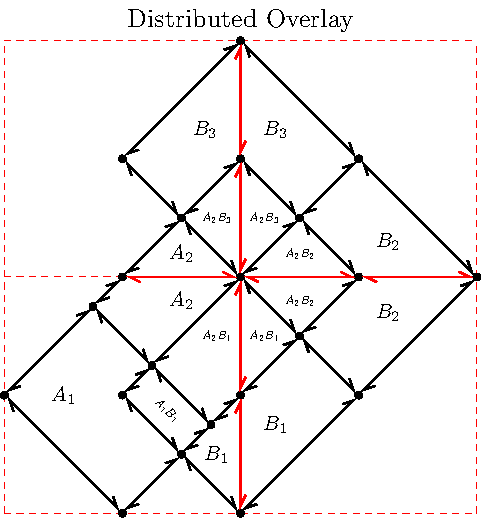
\includegraphics[scale=0.75]{overlay}};
    \node[scale=2] at (4,-3.25)    {$\Longrightarrow$};
    \node at (8,-3) {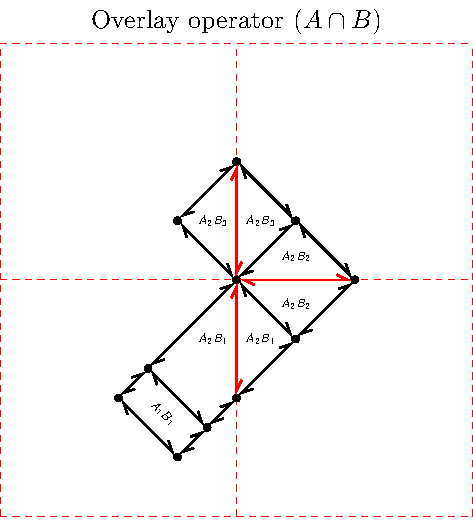
\includegraphics[scale=0.75]{operator}};
    \node[scale=2] at (12,-3.25)    {$\Longrightarrow$};
    \node at (16,-3) {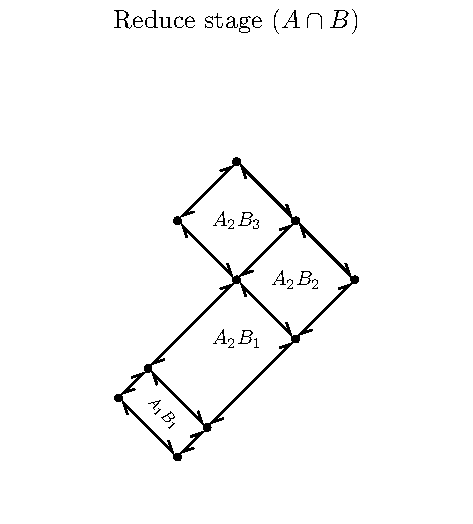
\includegraphics[scale=0.75]{reduce}};
    \node[scale=1.5] at (0,-7) {(a)};
    \node[scale=1.5] at (8,-7) {(b)};
    \node[scale=1.5] at (16,-7) {(c)};
\end{tikzpicture}
\end{document}
